\subsubsection{Transformer Fine-Tuning}

Transformer models are fine-tuned using a standardized and conservative
setup, consistent with common practices in document classification.
Given the large training set and the use of pre-trained language models,
training is limited to 2--4 epochs to ensure convergence while avoiding
overfitting and unnecessary computational overhead.
Learning rates are selected from widely adopted fine-tuning ranges to
guarantee stable optimization.

Batch size is fixed by hardware constraints and not treated as a tunable
parameter. To account for stochastic effects, each configuration is
evaluated across multiple random seeds (noseed, 42, 1337, 2024).

\paragraph{Intra-seed Stability}
Stability with respect to random initialization is assessed by measuring
prediction agreement across different seeds, since ground-truth labels
are unavailable for the evaluation set.
High agreement across all architectures indicates stable convergence and
limited sensitivity to stochastic optimization.

\begin{table}[h]
\centering
\caption{Intra-seed prediction agreement for transformer models.}
\label{tab:intra_seed_agreement}
\small
\begin{tabular}{lccc}
\hline
\textbf{Model} & \textbf{Mean Agreement} & \textbf{Std} & \textbf{\#Seeds} \\
\hline
DeBERTa-512  & 0.8968 & 0.0011 & 3 \\
DeBERTa-256  & 0.9073 & 0.0009 & 3 \\
RoBERTa-512  & 0.9114 & 0.0004 & 3 \\
RoBERTa-256  & 0.9112 & 0.0001 & 3 \\
\hline
\end{tabular}
\end{table}

\paragraph{Cross-Architecture Hard-Case Analysis}
To assess architectural complementarity, prediction overlap is analyzed
on a subset of hard cases, defined as samples consistently misclassified
by simpler models.
High cross-architecture agreement on these samples suggests that residual
errors are driven by intrinsic semantic ambiguity rather than
hyperparameter choices or model-specific artifacts.

\begin{figure}[t]
	\centering
	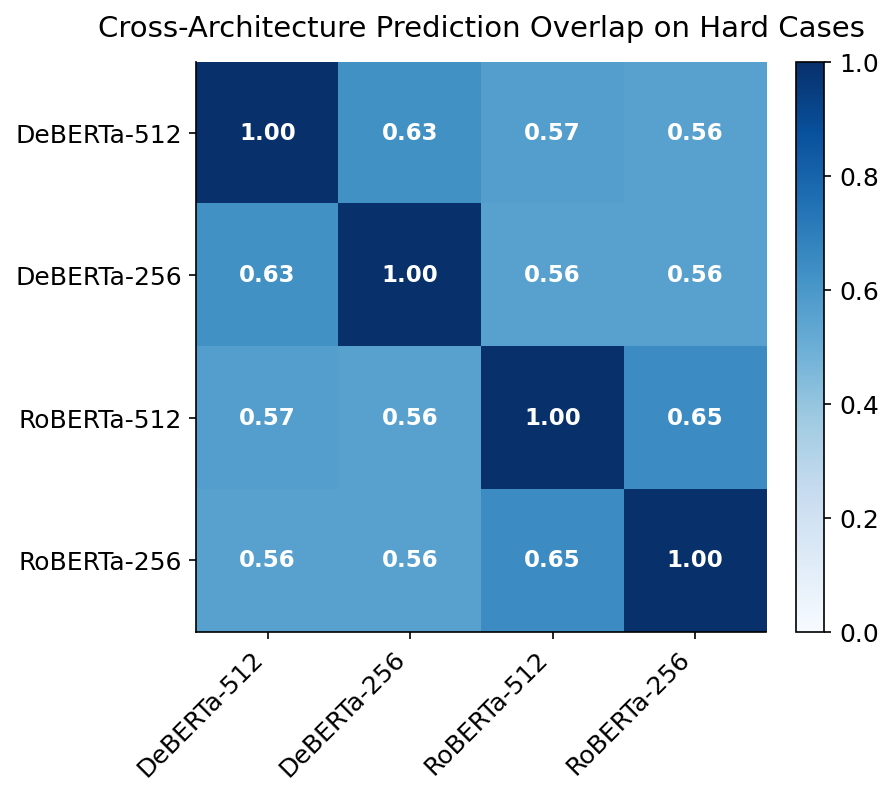
\includegraphics[width=0.75\linewidth]{FIGURES/overlap_hardcase}
	\caption{Cross-architecture prediction agreement on hard cases.
	Agreement is computed on samples with model disagreement, highlighting
	residual semantic ambiguity across transformer architectures.}
	\label{fig:cross_arch_overlap_hard}
\end{figure}

Overall, these analyses indicate that transformer fine-tuning operates in
a stable regime, with performance differences primarily determined by
architectural inductive biases rather than aggressive hyperparameter
optimization. Transformer models are therefore treated as robust semantic
baselines, whose complementarity is later exploited through ensemble
analysis.

